{
\setbeamertemplate{navigation symbols}{}
\setbeamercolor{background canvas}{bg={black}}
\color{white}
\begin{frame}[plain]
\fontsize{36pt}{36pt}\selectfont
\center
\begin{center}
Refactored Registration Framework
\end{center}

\fontsize{12pt}{12pt}\selectfont
\begin{center}
Insight Software Consortium
\end{center}
\newline
\begin{center}
 PICSL @ University of Pennsylvania 
\end{center}
\newline
\begin{center}
 Brian Avants, Nicholas Tustison, Gang Song, \\ 
Baohua Wu, Michael Stauffer, James C. Gee
\end{center}
\end{frame}
}

\begin{frame}
\frametitle{What is registration?}
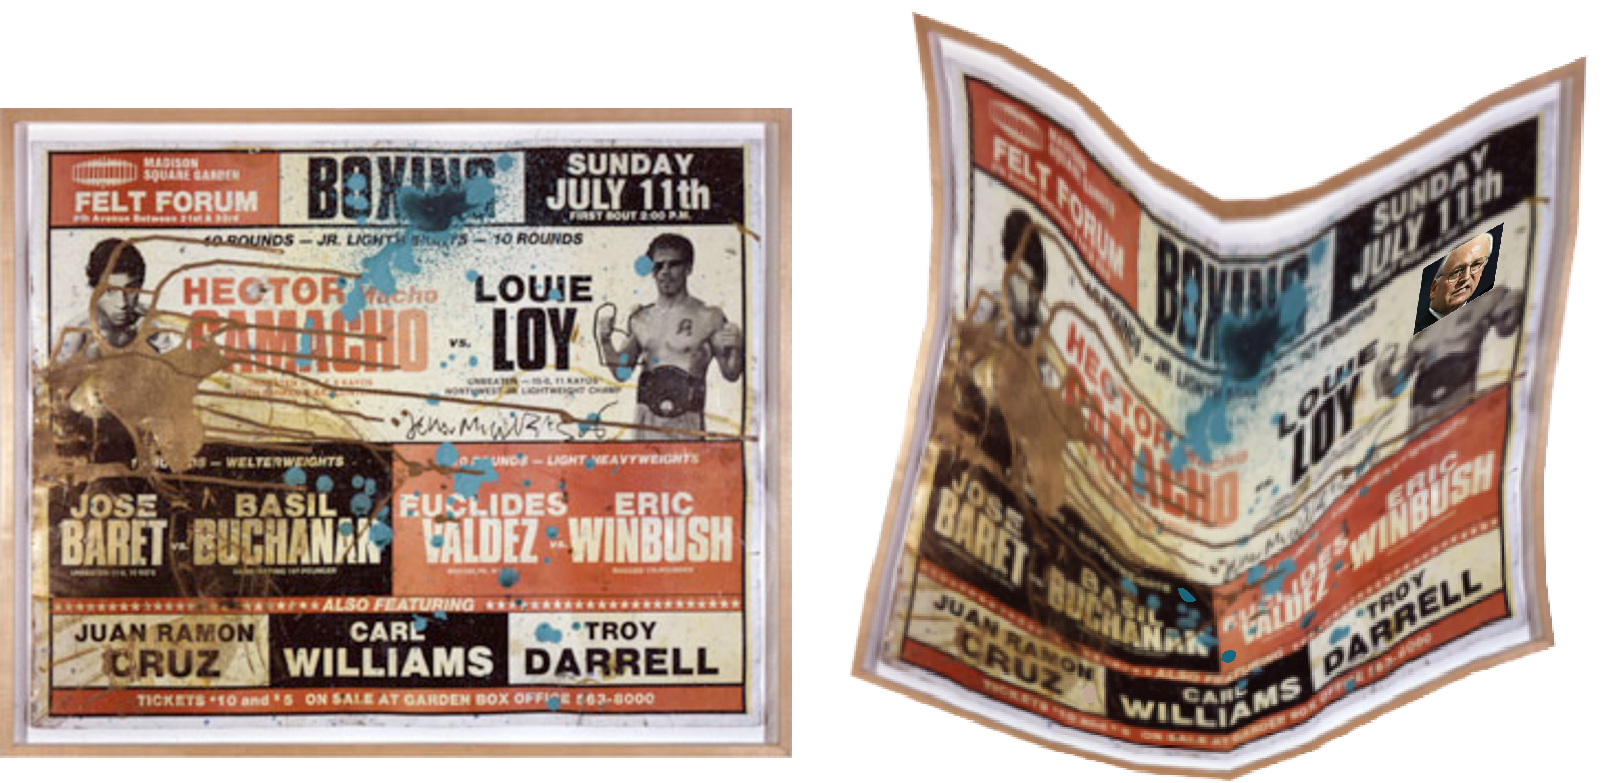
\includegraphics[height=2in]{../Art/RegistrationBasquiatWarp.pdf}
\end{frame}

\begin{frame}
\frametitle{What is registration?}
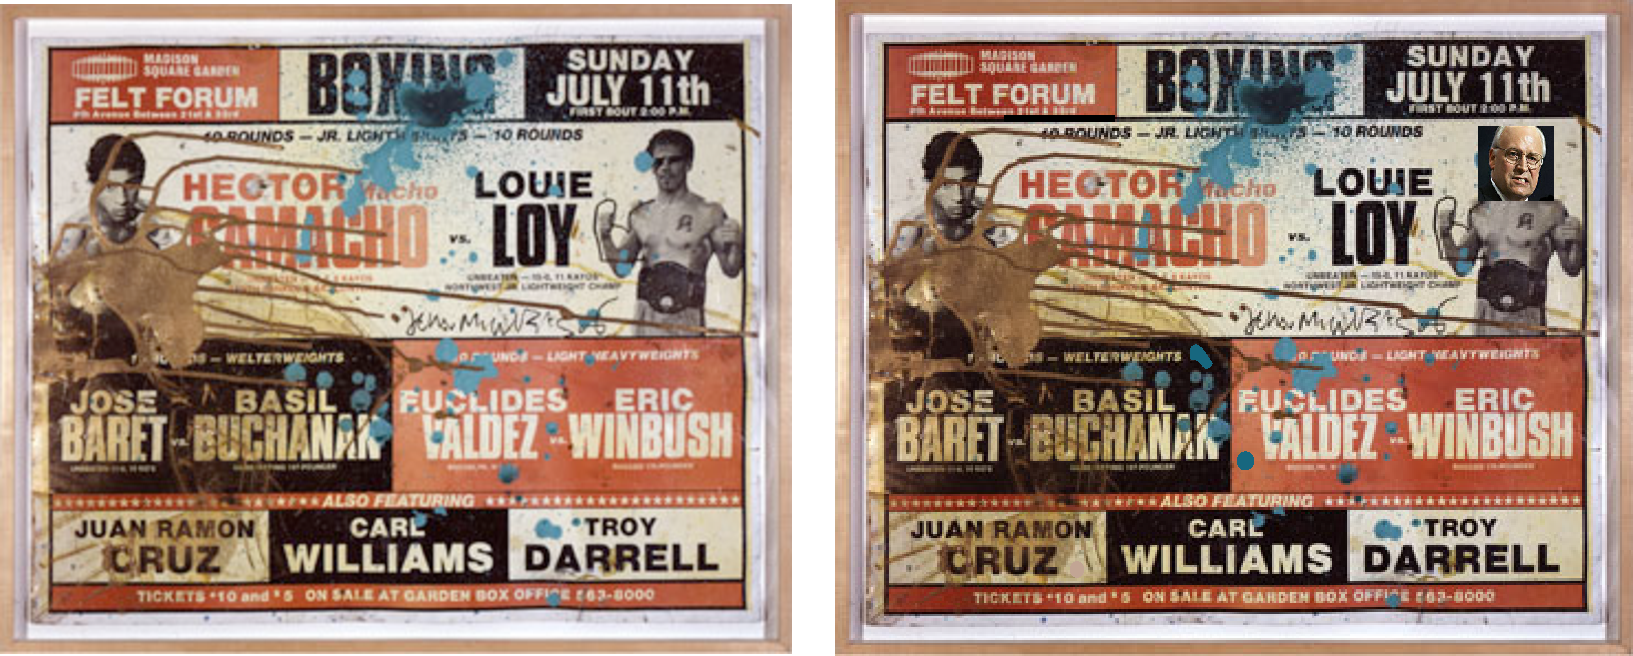
\includegraphics[height=1.8in]{../Art/RegistrationBasquiatDeWarp.pdf}
\end{frame}

\setbeamertemplate{background}{
\includegraphics[width=\paperwidth]{../Art/ITKv4_transparent}}

 \centeredlargetext{white}{black}{
\centering Enhanced user experience
%\newline
%
\includegraphics[height=1.8in]{../Art/ITKv4}
 }

 \centeredlargetext{white}{black}{
\centering Unified multi-core framework + parameter-estimation
%\newline
% 
\includegraphics[height=1.8in]{../Art/ITKv4}
 }

\begin{comment}
{

\begin{frame}
\frametitle{Image Registration Refactoring}
\Large
\begin{itemize}
\item Unify frameworks: local \& global 
\pause
\item New metrics and transform operations for vectors \&  tensors
\pause 
\item Composite Transform
\pause
\item Unbiased registration
\pause
\item Multi-threading 
\pause 
\item Automated parameter scaling
\end{itemize}
\end{frame}

\begin{frame}
\frametitle{Unified framework}
\Large
\begin{itemize}
\item Local \& global transforms treated the same in resampler
\item Both types available to (revised) optimizers
\item Revised metrics optimized for these operations
\item Tensors, vector, scalars treated transparently
\end{itemize}
\end{frame}
}
\end{comment}

 \centeredlargetext{white}{black}{
ITK v3 framework
\newline
\newline
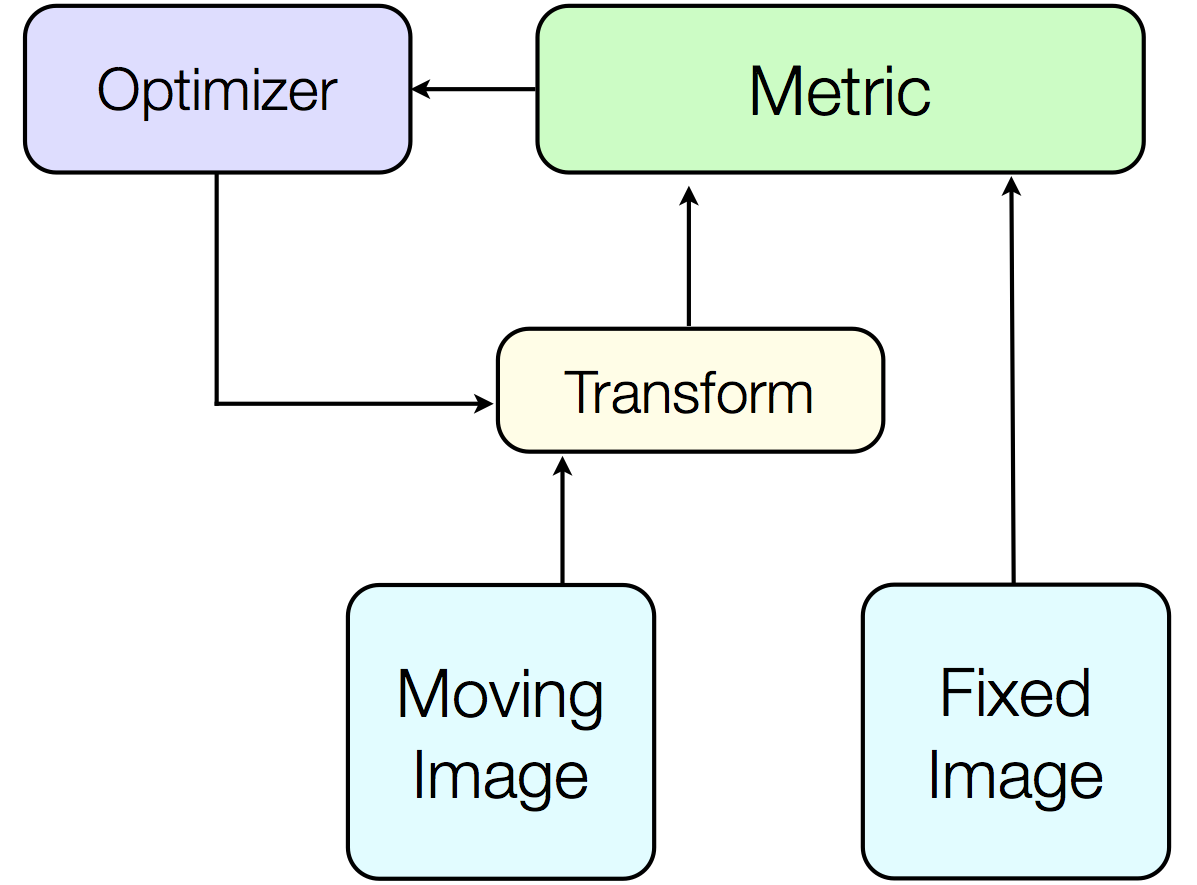
\includegraphics[height=2.2in]{../Art/itkv3reg}
 }

 \centeredlargetext{white}{black}{
ITK v4 framework
\newline
\newline
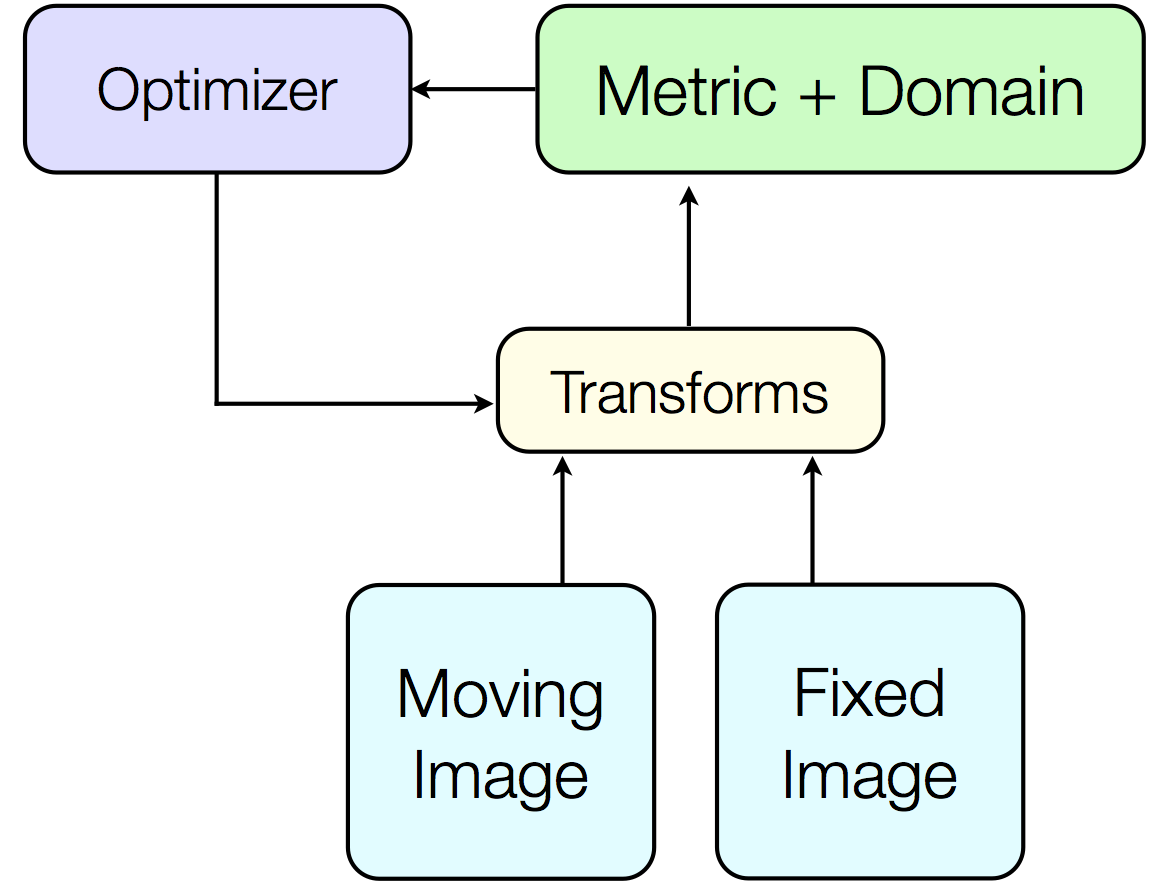
\includegraphics[height=2.2in]{../Art/itkv4reg}
 }

 \centeredlargetext{white}{black}{
\centering Compile external registration module
}

\begin{frame}
\frametitle{Compile external module}
\begin{itemize}
\item We link the external module
\lstlistingwithnumber{4}{5}{install_registration_code.cxx}
\item We recompile
\lstlistingwithnumber{6}{9}{install_registration_code.cxx}
\end{itemize}
\end{frame}


\begin{frame}
\frametitle{Image Registration Refactoring Example}
\end{frame}

\begin{frame}
\frametitle{Image Registration Refactoring Example}
ITK v4 Application
\end{frame}



\begin{frame}
\frametitle{New metrics}
\Large
\begin{itemize}
 sparse and dense neighborhood correlation
mutual information thevenaz
point sets ---  euclidean, pse, Jensen-Havrda-Charvat-Tsallis (JHCT)
tensor --- deviatoric 
vector --- arbitrary length
\end{itemize}
\end{frame}

\begin{frame}
\frametitle{Transform models}
\Large
\begin{itemize}
\item As v3 $+$ some new ones + thread safety 
\item displacement
\item bspline
\item polyaffine
\item diffeomorphism
\item velocityfield --- needs optimizer
\end{itemize}
\end{frame}

\begin{frame}
\frametitle{Multi-threading}
\Large
\begin{itemize}
\item code example
\end{itemize}
\end{frame}

\begin{frame}
\frametitle{Example registration}
\Large
\begin{itemize}
\item run the whole thing
\end{itemize}
\end{frame}

\begin{frame}
\frametitle{Parameter estimation }
\Large
\begin{itemize}
\item show parameter estimator 
\end{itemize}
\end{frame}

\begin{frame}
\frametitle{Thevenaz metric}
\Large
\begin{itemize}
\item X
\end{itemize}
\end{frame}

\centeredlargetext{black}{white}{
Registration\\
Parameter Tuning
}

\begin{frame}
\frametitle{Include Header Files}
\framesubtitle{itkThevenazMutualInformationImageToImageObjectRegistrationTest.cxx}
\begin{itemize}
\item We include ITK headers:
\lstlistingwithnumber{28}{33}{itkThevenazMutualInformationImageToImageObjectRegistrationTest.cxx}
\item We declare the components:
\lstlistingwithnumber{149}{155}{itkThevenazMutualInformationImageToImageObjectRegistrationTest.cxx}
\end{itemize}
\end{frame}



